\documentclass{beamer}

\newcommand{\lesson}{Algorithms}


\newcommand{\course}{Introduction to Object-Oriented Programming}
\subject{\course}
\title[\lesson]{\course}
\subtitle{\lesson}

\author[CS 1331]
{Christopher Simpkins \\\texttt{chris.simpkins@gatech.edu}}
\institute[Georgia Tech]

\date[]{}

\newcommand{\link}[2]{\href{#1}{\textcolor{blue}{\underline{#2}}}}
\newcommand{\code}{http://www.cs1331.org/code}

\usepackage{colortbl}

% If you have a file called "university-logo-filename.xxx", where xxx
% is a graphic format that can be processed by latex or pdflatex,
% resp., then you can add a logo as follows:

% \pgfdeclareimage[width=0.6in]{coc-logo}{cc_2012_logo}
% \logo{\pgfuseimage{coc-logo}}

\mode<presentation>
{
  \usetheme{Berlin}
  \useoutertheme{infolines}

  % or ...

 \setbeamercovered{transparent}
  % or whatever (possibly just delete it)
}

\usepackage{tikz}
% Optional PGF libraries
\usepackage{pgflibraryarrows}
\usepackage{pgflibrarysnakes}
\usepackage{pgfplots}
\usepackage{fancybox}
\usepackage{listings}
\usepackage{hyperref}
\hypersetup{colorlinks=true,urlcolor=blue}
\usepackage[english]{babel}
% or whatever

\usepackage[latin1]{inputenc}
% or whatever

\usepackage{times}
\usepackage[T1]{fontenc}
% Or whatever. Note that the encoding and the font should match. If T1
% does not look nice, try deleting the line with the fontenc.


\usepackage{listings}

% "define" Scala
\lstdefinelanguage{scala}{
  morekeywords={abstract,case,catch,class,def,%
    do,else,extends,false,final,finally,%
    for,if,implicit,import,match,mixin,%
    new,null,object,override,package,%
    private,protected,requires,return,sealed,%
    super,this,throw,trait,true,try,%
    type,val,var,while,with,yield},
  otherkeywords={=>,<-,<\%,<:,>:,\#,@},
  sensitive=true,
  morecomment=[l]{//},
  morecomment=[n]{/*}{*/},
  morestring=[b]",
  morestring=[b]',
  morestring=[b]""",
}

\usepackage{color}
\definecolor{dkgreen}{rgb}{0,0.6,0}
\definecolor{gray}{rgb}{0.5,0.5,0.5}
\definecolor{mauve}{rgb}{0.58,0,0.82}

% Default settings for code listings
\lstset{frame=tb,
  language=scala,
  aboveskip=2mm,
  belowskip=2mm,
  showstringspaces=false,
  columns=flexible,
  basicstyle={\scriptsize\ttfamily},
  numbers=none,
  numberstyle=\tiny\color{gray},
  keywordstyle=\color{blue},
  commentstyle=\color{dkgreen},
  stringstyle=\color{mauve},
  frame=single,
  breaklines=true,
  breakatwhitespace=true,
  keepspaces=true
  %tabsize=3
}


% \beamerdefaultoverlayspecification{<+->}

\begin{document}

\begin{frame}{}
%  \titlepage
\vspace{-.1in}
  \begin{center} 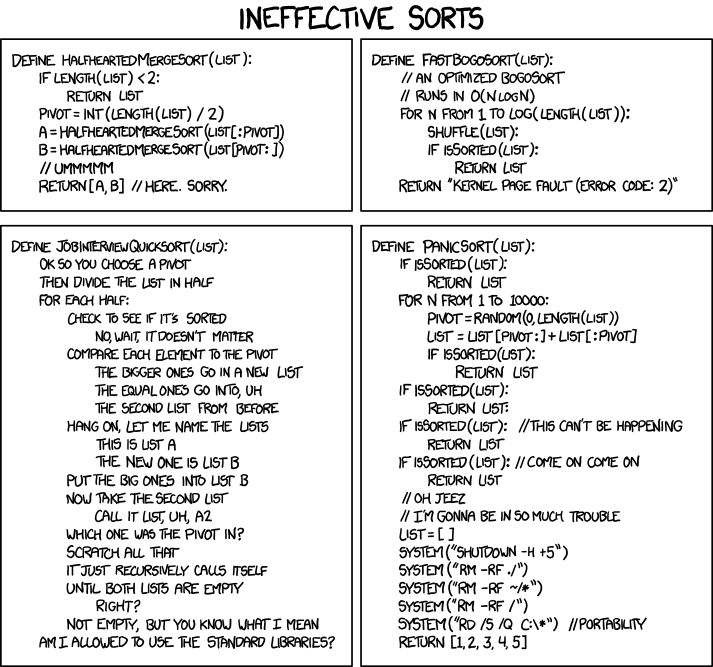
\includegraphics[height=3.2in]{ineffective_sorts.png}\footnote{\link{http://xkcd.com/1185/}{http://xkcd.com/1185/}}
  \end{center}
\end{frame}

\begin{frame}{}
\vspace{-.2in}
  \titlepage
\vspace{-.75in}
\begin{center}
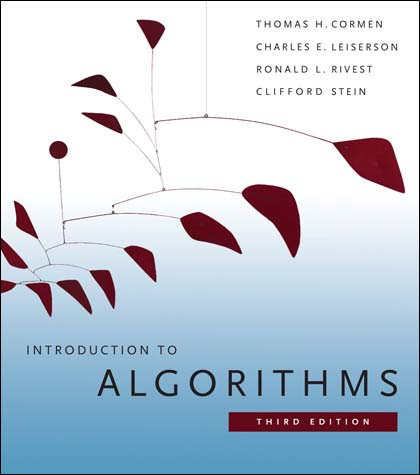
\includegraphics[height=1.75in]{clrs.jpg}\\
\link{http://mitpress.mit.edu/books/introduction-algorithms}{{\LARGE CLRS}}
\end{center}

\end{frame}


%------------------------------------------------------------------------
\begin{frame}[fragile]{Algorithms}

An {\it algorithm} is a sequence of operations that accomplishes a task, or solves a problem.  We demand that an algorithm be
\begin{itemize}
\item {\it correct} -- if the algorithm's input satisfies the algorithm's assumptions, the algorithm always produces correct output --
\end{itemize}
and want an algorithm to be
\begin{itemize}
\item {\it efficient} -- the algorithm uses the least amount of resources necessary to accomplish its task.
\end{itemize}

Today we'll learn how to analyze the efficiency of an algorithm in the context of two fundamental problems in computation: searching and sorting.  First we'll briefly touch on correctness using loop invariants.

\end{frame}
%------------------------------------------------------------------------

%------------------------------------------------------------------------
\begin{frame}[fragile]{The Sorting Problem}

Sorting means rearranging the elements of an array (or {\it permuting} the array) so that the elements are in a well-defined order.  For example, we can sort an array in non-decreasing order (ascending) so that each element $A[i] \le A[i + 1]$ for $i = 1 \ldots n - 1$.
% \begin{lstlisting}[language=Java]

% \end{lstlisting}

\begin{itemize}
\item Note that we don't define a separate output, only a result, or effect.
\end{itemize}

\begin{quote}
In today's discussion we'll assume that our input is an array whose elements are integers.  We've already seen how to generalize to arbitray user-defined types.
\end{quote}

\end{frame}
%------------------------------------------------------------------------

%------------------------------------------------------------------------
\begin{frame}[fragile]{Insertion Sort}


The insertion sort algorithm in pseudocode (from CLRS Chapter 2):
\vspace{-.05in}
\begin{lstlisting}[]
1 for j = 2 to A.length // A[1 .. A.length] is an array
2     key = A[j]
3     // Insert A[j] into the sorted sequence A[1 .. j - 1].
4     i = j - 1
5     while i > 0 and A[i] > key
6         A[i + 1] = A[i]
7         i = i - 1
8    A[i + 1] = key
\end{lstlisting}

Note the following conventions we use when describing algorithms abstractly:
\begin{itemize}
\item we use pseudocode instead of code in a particular programming language,
\item the array indices start at 1 instead of 0, and
\item the array has a property {\it length} so that we don't have to specify the array's size separately.
\end{itemize}

\end{frame}
%------------------------------------------------------------------------

%------------------------------------------------------------------------
\begin{frame}[fragile]{Loop Invariants}


A loop invariant expresses a formal property of an algorithm that:
\begin{itemize}
\item is true prior to the first iteration of the loop,
\item if it is true before an iteration of the loop remains true before the next iteration, and
\item upon loop termination gives a useful property that helps show that the algorithm is correct.
\end{itemize}


\end{frame}
%------------------------------------------------------------------------

%------------------------------------------------------------------------
\begin{frame}[fragile]{A Loop Invariant for Insertion Sort}

\begin{lstlisting}[]
1 for j = 2 to A.length
2     key = A[j]
3     // Insert A[j] into the sorted sequence A[1 .. j - 1].
4     i = j - 1
5     while i > 0 and A[i] > key
6         A[i + 1] = A[i]
7         i = i - 1
8    A[i + 1] = key
\end{lstlisting}

\begin{quote}
At the start of each iteration of the for loop of lines 1-8, the subarray A[1 .. j - 1] consists of the elements originally in A[1 .. j - 1], but in sorted order.
\end{quote}

\end{frame}
%------------------------------------------------------------------------

%------------------------------------------------------------------------
\begin{frame}[fragile]{Expresing Loop Invariants as {\tt assert}ions}

Insertion sort in Java (note translation to 0-based indexes):
\begin{lstlisting}[language=Java]
for (int j = 1; j < a.length; ++j) {
    assert isSorted(a, 0, j - 1);
    int key = a[j];
    int i = j - 1;
    while(i >= 0 && a[i] > key) {
        a[i + 1] = a[i];
        i = i - 1;
    }
    a[i + 1] = key;
}
\end{lstlisting}
Note that we didn't express the entire invariant in Java.  We could, but you must trade off implementation effort and benefit. Run the program with the {\tt -ea} switch to enable assertions:
\begin{lstlisting}[language=Java]
$ java -ea InsertionSort
\end{lstlisting}

See \link{\code/algorithms/InsertionSort.java}{InsertionSort.java}.


\end{frame}
%------------------------------------------------------------------------

%------------------------------------------------------------------------
\begin{frame}[fragile]{The Search Problem}

The search problem is defined formally by the following input-output specifications:
\begin{itemize}
\item Input: A sequence of $n$ elements $A = <a_1, a_2, ..., a_n>$ and a value $v$
\item Output: An index $i$ such that $v = A[i]$, or a special value such as -1 or $nil$ if $v$ does not appear in $A$.
\end{itemize}

We'll see that the assumptions we can make about the input affects the efficiency of the algorhtms we can use to search it.

\end{frame}
%------------------------------------------------------------------------


%------------------------------------------------------------------------
\begin{frame}[fragile]{Linear Search}

If we can make no assumptions about the order of the array, our only option is linear search:
\begin{lstlisting}
// A is an array, and v is the value we're searching for
LINEAR-SEARCH(A, v):
  for i = 1 to A.length
      if A[i] = v then
          return i
  return -1
\end{lstlisting}

We'll be dealing with search algorithms abstractly for the purpose of discussing running time analysis, but example implementations are available in \link{\code/algorithms/Search.java}{Search.java}.

\end{frame}
%------------------------------------------------------------------------

%% %------------------------------------------------------------------------
%% \begin{frame}[fragile]{Correctness of Linear Search}


%% \begin{lstlisting}[language=Java]

%% \end{lstlisting}

%% \begin{itemize}
%% \item
%% \end{itemize}


%% \end{frame}
%% %------------------------------------------------------------------------

%------------------------------------------------------------------------
\begin{frame}[fragile]{Algorithmic Efficiency}

We can characterize algorithmic efficiency in terms of space complexity (how much storage an algorithm requires) or time complexity (how ``fast'' an algorithm runs).  Almost always primarily concerned with time complexity.

\begin{itemize}
\item Note that we want to eliminate platform-specific factors, like speed of the particular computer an algorithm runs on.

\end{itemize}

So we characterize algorithm performance in terms of
\begin{itemize}
\item input size, $n$, and
\item order of growth as a function of input size.
\end{itemize}

An efficient algorithm beats an inefficient one even if the inefficient algortithm is run on a far superior computer.

\end{frame}
%------------------------------------------------------------------------

%------------------------------------------------------------------------
\begin{frame}[fragile]{Efficiency of Linear Search}

Assuming each operation has a fixed cost, we can count the operations performed for a worst-case input as follows:\\
\vspace{.1in}
\begin{tabular}{lll}
Step                         & Cost  & Times \\\hline
\verb@for i = 1 to A.length@ & $c_1$ & $n$ \\
\verb@    if A[i] = v then@  & $c_2$ & $n$ \\
\verb@        return i@      & $c_3$ & $0$ \\
\verb@return -1@             & $c_4$ & $1$ \\
\end{tabular}\\
\vspace{.1in}
Adding up the number of times each statement is executed we get:
\[
T(n) = c_1n + c_2n + c_4 = (c_1 + c_2)n + c_4
\]
We discard contant terms, constant factors, and lower-order terms to say that the worst case running time is
\[
O(n)
\]
And pronounce this ``order n'' or ``Big-O of n.''

\end{frame}
%------------------------------------------------------------------------

%------------------------------------------------------------------------
\begin{frame}[fragile]{Binary Search}

\vspace{-.05in}
If the array is sorted you can use a binary search:
\vspace{-.05in}
\begin{lstlisting}[mathescape]
BINARY-SEARCH(A, v):
  p := 1, r := A.length
  while p $\le$ r
      q := $\lfloor{(p+r)/2\rfloor}$
      if A[q] = v then
          return q
      if A[q] > v then
          r := q - 1
      else
          p = q + 1
  return -1
\end{lstlisting}
\vspace{-.05in}
Intuitively: We check the midpoint of the array (q).
\begin{itemize}
\item If the array is empty (p > r), the query value was not found.
\item If the midpoint holds the value, return the midpoint.
\item If the midpoint holds a value greater than our search value, repeat the process with the lower half of the array.
\item If the midpoint holds a value less than our search value, repeat the process with the upper half of the array.
\end{itemize}

\end{frame}
%------------------------------------------------------------------------

%------------------------------------------------------------------------
\begin{frame}[fragile]{Efficiency of Binary Search}

The key to analyzing the efficiency of BINARY-SEARCH is realizing that the array is halved in each iteration of the while loop.
\begin{itemize}
\item In the worst case BINARY-SEARCH runs until the size of the array ($r-p$) goes from $n$ to $1$ by successive halving.
\item This is equivalent to going from $1$ to $n$ by successive doubling.
\end{itemize}
Counting the number of times $x$ we need to double to get from $1$ to $n$ is
\[
2^x = n
\]
so
\[
x = \lg n
\]
and the worst-case running time of BINARY-SEARCH is\\
\[
O(\lg n)
\]

\end{frame}
%------------------------------------------------------------------------

%------------------------------------------------------------------------
\begin{frame}[fragile]{Efficiency of Insertion Sort (Worst Case)}


\begin{tabular}{lll}
Step                                   & Cost  & Times \\\hline
\verb@1: for j = 2 to A.length         @  & $c_1$ & $n$ \\
\verb@2:     key = A[j]@                  & $c_2$ & $n - 1$  \\
\end{tabular}
\verb@ 3:     @// Insert A[j] into sorted A[i .. j - 1].\\
\begin{tabular}{lll}
\verb@4:     i = j - 1@                   & $c_4$ & $n - 1$  \\
\verb@5:     while i > 0 and A[i] > key@  & $c_5$ & $\sum_{j=2}^n j$  \\
\verb@6:         A[i + 1] = A[i]@         & $c_6$ & $\sum_{j=2}^n (j - 1)$  \\
\verb@7:         i = i - 1@               & $c_7$ & $\sum_{j=2}^n (j - 1)$  \\
\verb@8:    A[i + 1] = key@               & $c_8$ & $n - 1$  \\
\end{tabular}
\\
\vspace{.1in}
Noting the sum of the arithmetic series $\sum_1^n x = \frac{n(n-1)}{2} = \frac{1}{2}n(n+1)$, adding the running times, simplifying, discarding constant terms and factors, and lower-order terms we get:
\[
O(n^2)
\]


\end{frame}
%------------------------------------------------------------------------


%------------------------------------------------------------------------
\begin{frame}[fragile]{Run-time Analysis Summary: Linear}

Sample pseudocode:
\begin{lstlisting}[language=Python]
for i := 1 to n
    // ...
\end{lstlisting}
Java implementation:
\begin{lstlisting}[language=Java]
for (int i = 0; i < n; i++) {
    // ...
}
\end{lstlisting}
Intuition:
\begin{itemize}
\item ``For each of the $n$ elements,'' or ``for $n$ times.''
\end{itemize}
Big-O:
\[
O(n)
\]

\end{frame}
%------------------------------------------------------------------------

%------------------------------------------------------------------------
\begin{frame}[fragile]{Run-time Analysis Summary: Quadratic}

Sample pseudocode:
\begin{lstlisting}[language=Python]
for i := 1 to n
    for j := 1 to n
\end{lstlisting}
Java implementation:
\begin{lstlisting}[language=Java]
for (int i = 0; i < n; i++) {
    for (int j = 0; j < n; j++) {
        // ...
    }
}
\end{lstlisting}
Intuition:
\begin{itemize}
\item ``$n$ times for each $n$''
\end{itemize}
Big-O:
\[
O(n^2)
\]

\end{frame}
%------------------------------------------------------------------------

%------------------------------------------------------------------------
\begin{frame}[fragile]{Run-time Analysis Summary: Also Quadratic}

Sample pseudocode:
\begin{lstlisting}[language=Python]
for i := 1 to n
    for j := 1 to i
\end{lstlisting}
Java implementation:
\begin{lstlisting}[language=Java]
for (int i = 0; i < n; i++) {
    for (int j = 0; j < i; j++) {
        // ...
    }
}
\end{lstlisting}
Intuition:
\begin{itemize}
\item For each $i = 1 .. n$, count up to $i$
\item This is sum of the the arithmetic series: $\sum_1^n x = \frac{n(n-1)}{2} = \frac{1}{2}n(n+1) = \frac{1}{2}n^2 + \frac{1}{2}n$
\end{itemize}
Big-O:
\[
O(n^2)
\]

\end{frame}
%------------------------------------------------------------------------

%------------------------------------------------------------------------
\begin{frame}[fragile]{Run-time Analysis Summary: Logarithmic (1 of 2)}
\vspace{-.05in}
Sample pseudocode:
\vspace{-.05in}
\begin{lstlisting}[language=Python,mathescape]
  p := 1, r := n
  while p $\le$ r
     // cut difference between p and r in half until it's 0...
\end{lstlisting}
\vspace{-.05in}
Java implementation:
\vspace{-.05in}
\begin{lstlisting}[language=Java]
  int lo = 0, hi = array.length - 1;
  while (lo <= hi) {
      int middle = (lo + hi)/2;
      // either lo becomes middle + 1, or hi becomes middle - 1
  }
\end{lstlisting}
\vspace{-.05in}
Intuition:
\vspace{-.05in}
\begin{itemize}
\item Each iteration of the loop cuts the remaining input in half.  We stop when we've cut the input size to 1.
\item Mathematically, we're multiplying the input size by $\frac{1}{2}$ each time.
\item Run-time is the number of times we multiply by $\frac{1}{2}$
\end{itemize}
Mathematically ...
\end{frame}
%------------------------------------------------------------------------

%------------------------------------------------------------------------
\begin{frame}[fragile]{Run-time Analysis Summary: Logarithmic (2 of 2)}

\vspace{-.05in}
\begin{lstlisting}[language=Python,mathescape]
  p := 1, r := n
  while p $\le$ r
     // cut difference between p and r in half until it's 0...
\end{lstlisting}
Run-time is the number of times $x$ we multiply by $\frac{1}{2}$:
\begin{align*}
\frac{1}{2^x}n  & = 1\\
\frac{1}{2^x}   & = \frac{1}{n}\\
2^x             & = n\\
x               & = \log_2 n
\end{align*}
So Big-O is:
\[
O(\log n)
\]

\end{frame}
%------------------------------------------------------------------------

%------------------------------------------------------------------------
\begin{frame}[fragile]{Closing Thoughts}


% \begin{lstlisting}[language=Java]

% \end{lstlisting}

\begin{itemize}
\item Algorithms and data structures are two sides of the same coin
\item Data structures affect the kinds of algorithms that can operate on the data
\item Operations on data structures are defined by algorithms
\item Abstract data types package data structures with their associated algorithms
\end{itemize}

\end{frame}
%------------------------------------------------------------------------

% %------------------------------------------------------------------------
% \begin{frame}[fragile]{}


% \begin{lstlisting}[language=Java]

% \end{lstlisting}

% \begin{itemize}
% \item
% \end{itemize}


% \end{frame}
% %------------------------------------------------------------------------



\end{document}
